\section{Arhitektura sustava i implementacija}
\label{chap:implementacija}
Nakon definiranja teorijskih osnova i formalizacije problema, ovo poglavlje detaljno opisuje praktičnu realizaciju razvijenog optimizacijskog modela. Sustav je implementiran u programskom jeziku Python (verzija 3.x), odabranom zbog čitljivosti, bogatog ekosustava biblioteka i široke primjene u znanstvenom računarstvu \cite{PythonSoftwareFoundation}. U nastavku se opisuje arhitektura programskog rješenja, korištene tehnologije te detalji implementacije ključnih komponenata.
\subsection{Korištene tehnologije i biblioteke}
Za izradu sustava korišten je niz standardnih biblioteka iz Python ekosustava za znanstveno računarstvo. Biblioteka DEAP \cite{DEAP2012} korištena je kao temeljni okvir za implementaciju genetskog algoritma. Za numeričke operacije i statističku obradu korišten je NumPy \cite{Harris2020}, dok je za manipulaciju i spremanje tabličnih podataka korišten Pandas \cite{PandasDevelopmentTeam2020}. Vizualizacija rezultata provedena je pomoću biblioteka Seaborn \cite{Waskom2021} i Matplotlib \cite{Hunter2007}. Modeliranje nesigurnosti pomoću Trokutaste distribucije implementirano je korištenjem standardne Python biblioteke Random. Detaljan pregled dan je u Tablici \ref{tab:biblioteke}.
\begin{table}[H]
\centering
\caption{Korištene biblioteke u implementaciji}
\label{tab:biblioteke}
\begin{tabular}{|l|p{10cm}|}
\hline
\textbf{Biblioteka} & \textbf{Namjena i citat} \\ \hline
Python & Osnovni programski jezik za cjelokupnu implementaciju. \cite{PythonSoftwareFoundation} \\ \hline
DEAP & Okvir za razvoj i provedbu evolucijskih algoritama. \cite{DEAP2012} \\ \hline
NumPy & Numeričke operacije i statistička obrada nizova podataka. \cite{Harris2020} \\ \hline
Pandas & Učitavanje, obrada i spremanje tabličnih podataka s rezultatima. \cite{PandasDevelopmentTeam2020} \\ \hline
Seaborn & Kreiranje naprednih statističkih vizualizacija (stupčasti, linijski i raspršeni grafikoni). \cite{Waskom2021} \\ \hline
Matplotlib & Osnovna biblioteka za crtanje na koju se oslanja Seaborn. \cite{Hunter2007} \\ \hline
Random & Standardna Python biblioteka korištena za generiranje slučajnih brojeva i uzorkovanje iz Trokutaste distribucije. \\ \hline
\end{tabular}
\end{table}

\subsection{Arhitektura eksperimentalnog okvira}

Sustav razvijen za potrebe ovog rada nije zamišljen kao monolitna skripta, već kao cjeloviti i modularni eksperimentalni okvir. Takva arhitektura, prikazana na Slici \ref{fig:tok_istrazivanja}, omogućuje sustavnu analizu, kalibraciju i usporedbu optimizacijskih metodologija kroz dvo-fazni proces istraživanja. Okvir se sastoji od dva glavna analitička modula koji slijede dvo-fazni pristup istraživanju, te jednog pomoćnog modula za obradu i prikaz rezultata.

Prvi modul, \textbf{Modul za analizu i kalibraciju genetskog algoritma}, predstavlja temelj istraživanja i odgovara na pitanje: \emph{``Kako optimalno konfigurirati genetski algoritam za rješavanje zadanog problema?''}. Njegova primarna svrha je provođenje detaljne ablacijske studije kojom se ispituje utjecaj svakog ključnog parametra na performanse. Kroz višestruka pokretanja različitih konfiguracija (standardni GA, bez križanja, bez mutacije, s povećanim brojem generacija, s većom populacijom), izračunavanjem metrika performansi, uključujući prosječnu vrijednost (mean) i standardnu devijaciju (std) za ROI i procijenjeno trajanje, ovaj modul kao izlaz generira "šampionsku" konfiguraciju – skup optimalnih parametara koji osiguravaju najbolje performanse i koji se koriste u daljnjoj analizi.

    Drugi, ključni modul je \textbf{Modul za usporednu analizu optimizacijskih scenarija}. On čini srž diplomskog rada i koristi "šampionsku" konfiguraciju za provođenje konačne, statistički robusne usporedbe triju različitih pristupa rješavanju problema: osnovnog modela nasumične pretrage, klasičnog genetskog algoritma usmjerenog isključivo na ROI, te hibridnog GA+MC modela (NSGA-II) koji provodi više-kriterijsku optimizaciju koja istovremeno maksimizira ROI i minimizira rizik trajanja procijenjen Monte Carlo simulacijom.  Izlaz ovog modula je konačna tablica s usporednim rezultatima performansii(ROI, trajanje) i stabilnosti(standardna devijacija) za svaki od triju scenarija.

    Treći, \textbf{Modul za obradu i vizualizaciju rezultata}, služi kao pomoćni alat za interpretaciju podataka dobivenih iz prva dva modula. Njegova funkcionalnost obuhvaća generiranje preglednih tablica pomoću biblioteke \texttt{pandas}, spremanje rezultata u CSV format te stvaranje grafičkih prikaza, kao što su stupčasti dijagrami za usporedbu prosječnih vrijednosti ili 2D raspršeni dijagrami za prikaz Paretovog fronta.
\begin{figure}[H]
    \centering
    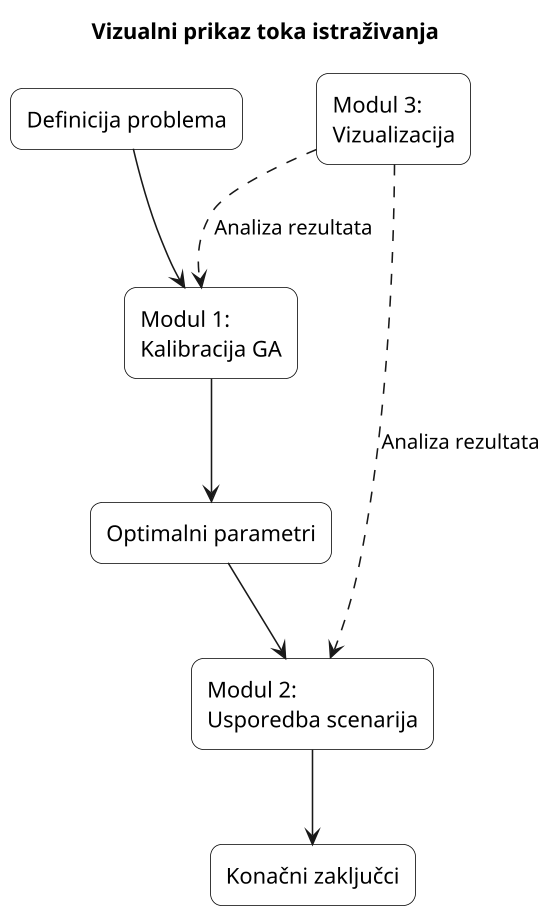
\includegraphics[width=0.9\textwidth]{slike/tijek_istrazivanja.png}
    \caption{Vizualni prikaz toka istraživanja}
    \label{fig:tok_istrazivanja}
\end{figure}
\subsection{Implementacija ključnih komponenti}
\subsubsection{Modeliranje nesigurnosti: Monte Carlo simulacija}

Za svaku projektnu aktivnost definirane su tri točke procjene trajanja:
\[
a \ (\text{optimistična}), \quad
m \ (\text{najvjerojatnija}), \quad
b \ (\text{pesimistična})
\]
Iako u teoriji postoje kompleksnije distribucije poput \textit{Beta-PERT} distribucije, 
za potrebe ovog rada odabrana je \textbf{Trokutasta distribucija (Triangular distribution)} 
zbog svoje praktičnosti, računalne efikasnosti i intuitivnog temelja na tri poznate procjene.

\paragraph{Generiranje trajanja aktivnosti.}
U svakoj iteraciji Monte Carlo simulacije, trajanje svake aktivnosti generira se slučajnom vrijednošću 
unutar raspona $[a, b]$ s najvećom vjerojatnošću u točki $m$.  
Trokutasta distribucija definirana je funkcijom gustoće vjerojatnosti:
\[
f(x) =
\begin{cases}
\frac{2(x-a)}{(b-a)(m-a)}, & a \leq x < m, \\
\frac{2(b-x)}{(b-a)(b-m)}, & m \leq x \leq b, \\
0, & \text{inače}.
\end{cases}
\]

\paragraph{Procjena trajanja portfelja.}
Ukupno trajanje projektnog portfelja u jednoj simulaciji dobiva se zbrojem trajanja svih aktivnosti odabranih u tom portfelju:
\[
T_{\text{portfolio}} = \sum_{i \in S} t_i
\]
gdje je $S$ skup odabranih aktivnosti, a $t_i$ generirano trajanje aktivnosti $i$.

Implementacija se temelji na \texttt{monte\_carlo\_eval\_duration} funkciji prikazanoj u Isječku koda \ref{lst:monte_carlo}, koja predstavlja konkretnu realizaciju teorijskog procesa opisanog u Poglavlju 2. Funkcija za zadani portfelj provodi velik broj simulacija (NUM_SIMULATIONS). U svakoj simulaciji, za svaku odabranu aktivnost generira se slučajno trajanje iz Trokutaste distribucije, zbrajaju se trajanja unutar te simulacije, a na kraju se vraća prosječna vrijednost svih simuliranih ukupnih trajanja.
\begin{lstlisting}[language=Python, caption={Funkcija za Monte Carlo procjenu trajanja}, label={lst:monte_carlo}, captionpos=b]
def monte_carlo_eval_duration(individual, activities, config):
    selected = [act for i, act in enumerate(activities) if individual[i] == 1]
    if not selected:
        return 0.0
    durations = [
        sum(
            random.triangular(act["optimistic"], act["realistic"], act["pessimistic"])
            for act in selected
        )
        for _ in range(config["NUM_SIMULATIONS"])
    ]
    return np.mean(durations)
\end{lstlisting}


\paragraph{Agregiranje rezultata.}
Monte Carlo simulacija ponavlja se velik broj puta $(\text{NUM\_SIMULATIONS})$, a konačna procjena trajanja portfelja 
dobiva se kao prosječna vrijednost svih simuliranih trajanja:
\[
\overline{T}(S) = \frac{1}{\text{NUM\_SIMULATIONS}} \sum_{k=1}^{\text{NUM\_SIMULATIONS}} T_{\text{portfolio}}^{(k)}
\]
gdje $T_{\text{portfolio}}^{(k)}$ označava ukupno trajanje portfelja u $k$-toj simulaciji.


\subsection{Optimizacijski pristup: Genetski algoritam}

Implementacija genetskog algoritma provedena je pomoću programske biblioteke \texttt{DEAP} (Distributed Evolutionary Algorithms in Python) \cite{DEAP2012}. 
S obzirom na prirodu problema odabira podskupa aktivnosti, korištena je \textbf{binarna reprezentacija}, gdje svaka jedinka (kromosom) predstavlja jedan portfelj projekata u obliku binarnog niza. Vrijednost '1' na poziciji i označava da je $i$-ta aktivnost odabrana, dok '0' označava da nije.
\paragraph{Reprezentacija jedinke.}
Svaka jedinka (kromosom) u populaciji predstavlja jedno potencijalno rješenje – jedan portfelj projekata. 
Predstavljena je kao binarni niz duljine jednake ukupnom broju aktivnosti $(\text{NUM\_ACTIVITIES})$, gdje gen na poziciji $i$ ima vrijednost:
\[
g_i =
\begin{cases}
1, & \text{ako je $i$-ta aktivnost odabrana}, \\
0, & \text{ako nije odabrana}.
\end{cases}
\]

\paragraph{Funkcija pogodnosti (Fitness Function).}
Ključni dio implementacije su funkcije pogodnosti. Ovisno o scenariju, korištene su dvije različite funkcije. Za jedno-kriterijsku optimizaciju (GA samo ROI), implementirana je funkcija koja maksimizira ROI i primjenjuje strogu kaznenu metodu za rješenja koja prekoračuju budžet, osiguravajući da su sva nevaljana rješenja lošija od bilo kojeg valjanog.
Za hibridni scenarij (GA+MC), implementirana je više-kriterijska funkcija pogodnosti koja predstavlja srž ovog rada. Kao što je prikazano u Isječku koda \ref{lst:fitness_function}, ova funkcija unutar jedne evaluacije objedinjuje deterministički izračun (ukupni trošak i ROI) i poziv stohastičke Monte Carlo simulacije za procjenu rizika (očekivano trajanje). Vraća tuple s dvije vrijednosti, omogućujući NSGA-II algoritmu da istovremeno optimizira oba cilja.
\begin{figure}
    \centering
\begin{lstlisting}[language=Python, caption={Više-kriterijska funkcija pogodnosti}, label={lst:fitness_function}, captionpos=b ]
def multi_objective_fitness(individual, activities, config):
    total_cost, total_roi = calculate_metrics(individual, activities)
    if total_cost > config["BUDGET"]:
        return 0, 99999
    avg_duration = monte_carlo_eval_duration(individual, activities, config)
    return total_roi, avg_duration
\end{lstlisting}
\end{figure}
Ovisno o eksperimentalnom scenariju, korištene su dvije vrste funkcije pogodnosti:
\begin{enumerate}
    \item \textbf{Jedno-kriterijska optimizacija.}  
Za scenarij GA (samo ROI), cilj je bio isključivo maksimizacija ukupnog povrata na investiciju (ROI). Za rukovanje ograničenjem budžeta primijenjena je stroga kaznena metoda. Ako ukupni trošak odabranog portfelja $S$ ne prelazi budžet, njegova pogodnost je jednaka ukupnom ROI-u. U suprotnom, pogodnost postaje negativna vrijednost proporcionalna iznosu prekoračenja:
$$
\text{Fitness}(S) = 
\begin{cases}
    \sum_{i \in S} \text{ROI}_i, & \text{ako } \sum_{i \in S} \text{Trošak}_i \leq \text{Budžet} \\
    -\left(\sum_{i \in S} \text{Trošak}_i - \text{Budžet}\right), & \text{ako } \sum_{i \in S} \text{Trošak}_i > \text{Budžet}
\end{cases}
$$
Ovakav pristup osigurava da svako valjano rješenje (koje ima pozitivan fitness) uvijek bude ocijenjeno kao bolje od bilo kojeg nevaljanog rješenja (koje ima negativan fitness).    \item \textbf{Više-kriterijska optimizacija.}  
    Za hibridni scenarij \texttt{GA+MC} korišten je napredni algoritam NSGA-II, s ciljem istovremene optimizacije dva suprotstavljena kriterija:
    \begin{enumerate}
        \item maksimizirati ROI,
        \item minimizirati prosječno trajanje projekta, procijenjeno Monte Carlo simulacijom.
    \end{enumerate}
    Formalno:
    \[
    \begin{cases}
    \max f_1(S) = ROI(S) \\
    \min f_2(S) = \overline{T}(S)
    \end{cases}
    \]
    gdje $\overline{T}(S)$ označava prosječno trajanje portfelja $S$.
\end{enumerate}

\paragraph{Genetski operatori.}
Za evoluciju populacije korišteni su sljedeći standardni genetski operatori za binarnu reprezentaciju koje pruža DEAP. Za \textbf{Selekciju} su primijenjeni Turnirska selekcija (\texttt{tools.selTournament}) za jedno-kriterijsku optimizaciju, te \texttt{tools.selNSGA2} za više-kriterijsku optimizaciju. Kao operator \textbf{križanja} korišteno je križanje u dvije točke (\texttt{tools.cxTwoPoint}), koje razmjenjuje segmente između dva roditeljska kromosoma, dok je za \textbf{mutaciju} korištena slučajna promjena bita (\texttt{tools.mutFlipBit}), koja s malom vjerojatnošću mijenja vrijednost pojedinog gena (iz $0$ u $1$ ili obrnuto), osiguravajući genetsku raznolikost i sprječavajući preranu konvergenciju.

\subsection{Vizualizacija i obrada rezultata}

Za analizu i prikaz rezultata dobivenih optimizacijom korištene su biblioteke \texttt{pandas} za tabličnu obradu podataka te \texttt{Seaborn} i \texttt{Matplotlib} \cite{Waskom2021, Hunter2007} za grafičku vizualizaciju.
Ovaj pristup omogućio je sustavnu prezentaciju statistički obrađenih podataka kroz detaljne tablice te vizualnu usporedbu modela pomoću stupčastih i raspršenih dijagrama. Posebno je značajan prikaz Paretovog fronta, koji jasno ilustrira kompromis (trade-off) između maksimizacije ROI-a i minimizacije trajanja, pružajući intuitivan uvid u kvalitetu rješenja dobivenih više-kriterijskom optimizacijom.

Kombinacija alata omogućila je jasnu i preglednu prezentaciju rezultata 
dobivenih iz eksperimentalnih scenarija.

Ključni vizualni elementi korišteni u ovom radu uključuju:

    \textbf{Tablične prikaze:} Detaljne tablice s konačnim, statistički obrađenim rezultatima 
    usporedbe različitih optimizacijskih scenarija, uključujući osnovne metrike 
    poput prosječnog ROI-a, prosječnog trajanja te raspona vrijednosti.

    \textbf{Stupčaste dijagrame:} Koristili su se za vizualnu usporedbu prosječnih vrijednosti 
    (\textit{ROI} i trajanje) između različitih metodologija optimizacije, omogućujući brzu identifikaciju 
    učinkovitijih pristupa.

    \textbf{Raspršene dijagrame (Scatter Plot):} Prikaz Paretovog fronta dobivenog NSGA-II algoritmom, 
    koji jasno ilustrira kompromis (\textit{trade-off}) između dvaju suprotstavljenih ciljeva:
    maksimizacije ROI-a i minimizacije trajanja. Time se omogućuje intuitivna procjena 
    učinkovitosti rješenja.

Vizualizacija rezultata odigrala je ključnu ulogu u interpretaciji dobivenih podataka, 
posebno u scenarijima s više ciljeva, gdje tablični prikazi sami po sebi nisu dovoljni 
za uočavanje odnosa i kompromisa među varijablama.

